\documentclass{article}
\usepackage{siunitx}
%% Language and font encodings
\usepackage[english]{babel}
\usepackage[utf8x]{inputenc}
\usepackage[T1]{fontenc}
\usepackage{longtable}
\usepackage{multirow}

%% Sets page size and margins
\usepackage[a4paper,top=3cm,bottom=2cm,left=3cm,right=3cm,marginparwidth=1.75cm]{geometry}

%% Useful packages
\usepackage{amsmath}
\usepackage{graphicx,float}
\usepackage[colorinlistoftodos]{todonotes}
\usepackage[colorlinks=true, allcolors=blue]{hyperref}

\title{CSP334: Computer Networks \linebreak
Lab Assignment No 2 \linebreak
Assignment on Linux Networking Commands}
\author{Abhishek Gupta  2016UCS0012}

\begin{document}
\maketitle


\section{Q1: Examine the following files in Linux}

\subsection{/etc/hosts}
As your machine gets started, it will need to know the mapping of some hostnames to IP addresses before DNS can be referenced. This mapping is kept in the /etc/hosts file. In the absence of a name server, any network program on your system consults this file to determine the IP address that corresponds to a host name.
\subsection{/etc/sysconfig/network}
The /etc/sysconfig/network file is used to specify information about the desired network configuration.It has the following values - Networking (yes or
no), Hostname, Gateway (IP address of network’s gateway) etc.
\subsection{/etc/sysconfig/network-scripts/ifcfg-eth0}
ifcfg-eth0  controls the first Ethernet network interface card or NIC in the system. In a system with multiple NICs, there are multiple ifcfg-eth<X> files (where <X> is a unique number corresponding to a specific interface).
\subsection{/etc/default-route}
This file contains the information about default-route. As we know
when a packet comes to a router it find the best route to the destination
(i.e. where the traffic is minimum) for that packet. When router was
unable to find any specific route the packet go through this default
route.
\subsection{/etc/resolv.conf}
resolv.conf is the name of a computer file used in various operating systems to configure the system's Domain Name System resolver.This resolver help in extractiong IP address from domain names which were sent from our system. This file
contain the search domain and the IP address of the DNS server.
\subsection{/etc/nsswitch.conf}
/etc/nsswitch.conf, is used by the GNU C Library to determine the sources from which to obtain name-service information in a range of categories, and in what order. Each category of information is identified by a database name. 

\section{Q2: Info about /etc/services File}
Services file at /etc/services stores information about numerous services that client applications might use on the computer. Within the file is the service name, port number and protocol it uses, and any applicable aliases.Transport Layer in the TCP/IP protocol stack make use of this file.The port numbers shown in this file are well-known port numbers. These are so becuase user can be sure not to use these port numbers while providing services to others.

\section{Q3: MAN Pages}
\begin{center}
 \begin{tabular}{| | m{2cm} | m{4cm} |  m{4cm} | m{4cm} | |} 
 \hline
 commandname & Purpose & Transportlayerprotocol & Networklayerprotocol \\ 
 \hline\hline
 arp & It maps IP Address to Physical Address on local network & NA & ARP \\ 
 \hline
 arping & It is a tool for probing host on network,it may use utility arp to resole IP Adress & NA & ARP \\
 \hline
 ifconfig & It displays status of currently active network interfaces and used to set interfaces in kernel &  &  \\
 \hline
 tcpdump & It provides description of the content of packets on a given network nterface &  &  \\
 \hline
 ping & It Exchange packets between two host and measure strength of connection btw client and server &  & ICMP \\
 \hline
 netstat & It prints list of networking subsystems by default it displays list of all open sockets &  &  \\
 \hline
route & It controls Kernel IP routing tables and it route to specific network or host which has been configured with terminal &  &  \\ 
 \hline
\end{tabular}
\end{center}

\section{Q4: TCPDUMP TRAFFIC}
tcpdump hostname remotehostname and localhostname \\
tcpdump hostname remotehostIP and localhostIP 
 \begin{figure}[H]
 \centering
 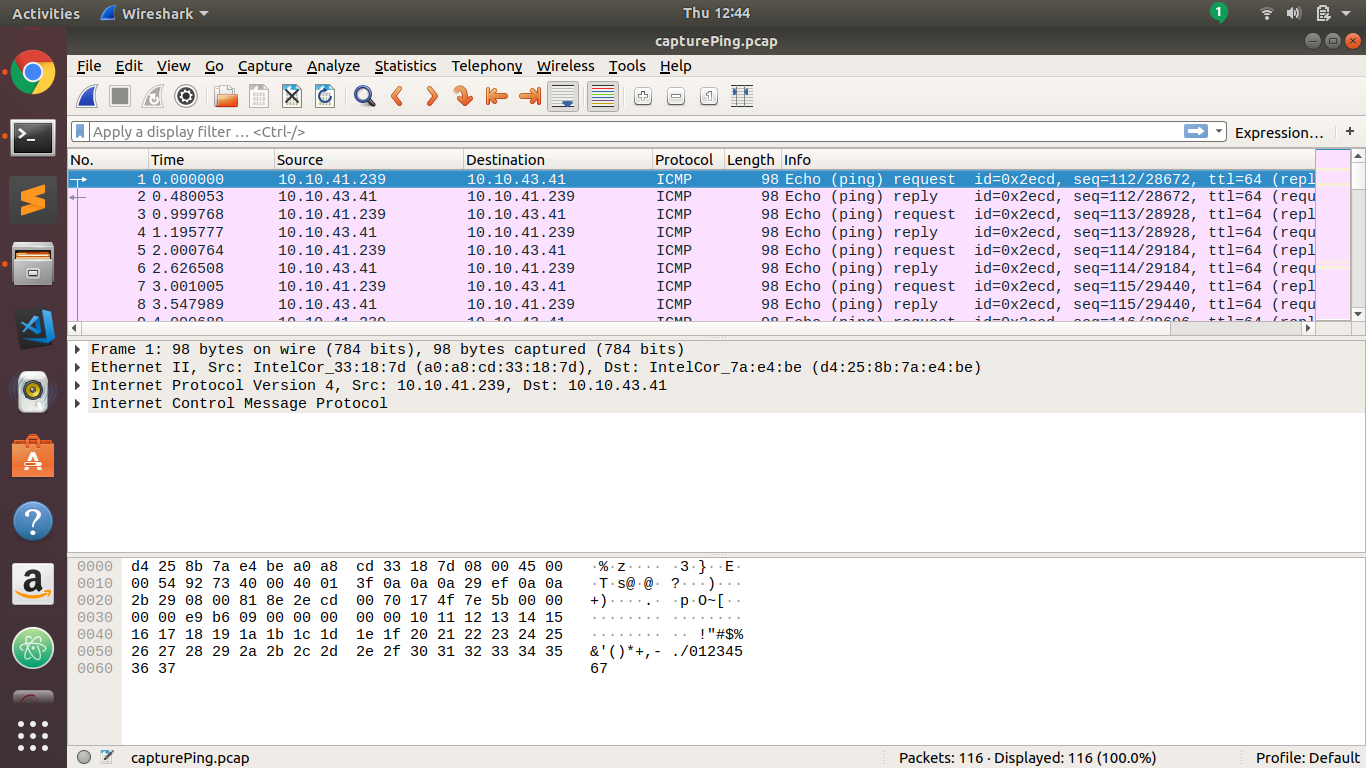
\includegraphics[width=1.0\textwidth]{../Q4/Ping.png}
 \caption{\label{fig:PING}Screenshot of tcpdump file}
 \end{figure}

\subsection{Request}
 \begin{figure}[H]
 \centering
 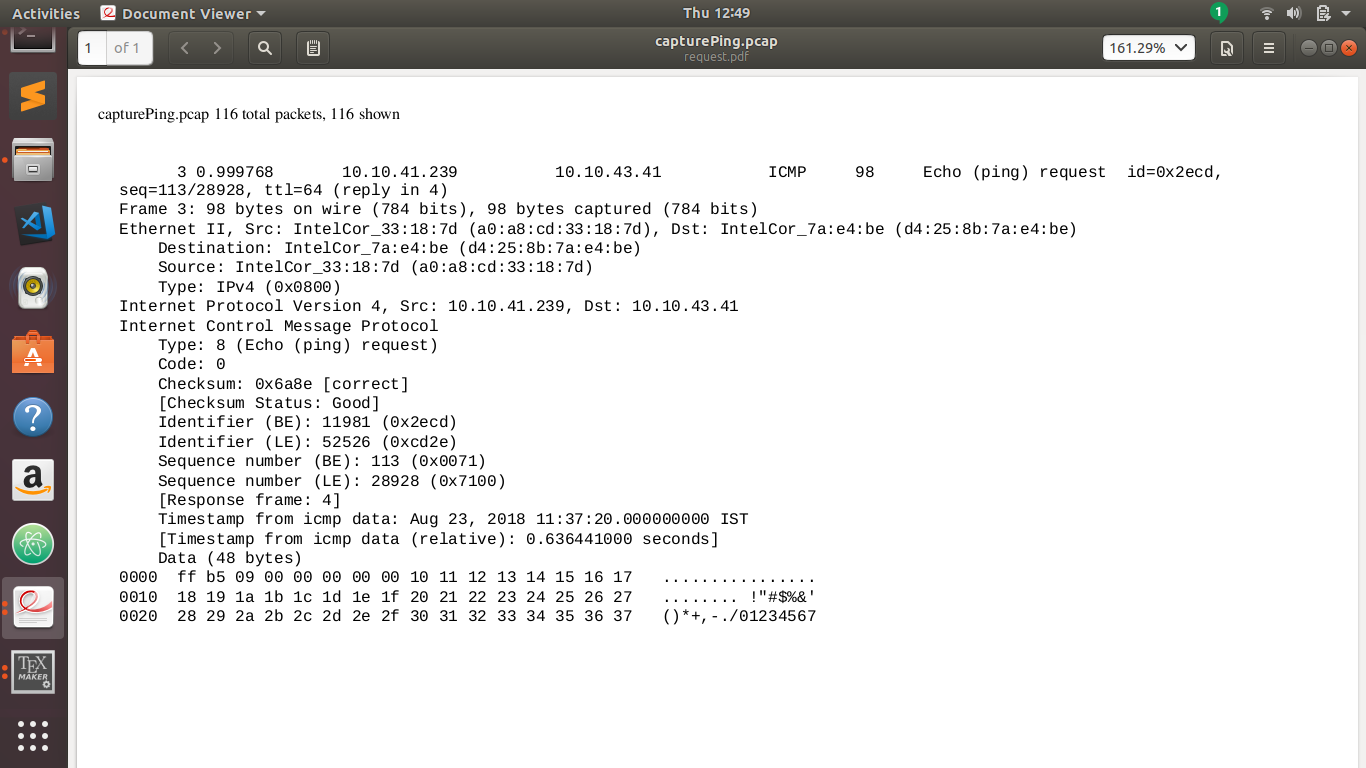
\includegraphics[width=0.7\textwidth]{../Q4/request.png}
 \caption{\label{fig:REQUEST}Ping Request.}
 \end{figure}

\subsection{Response}
 \begin{figure}[H]
 \centering
 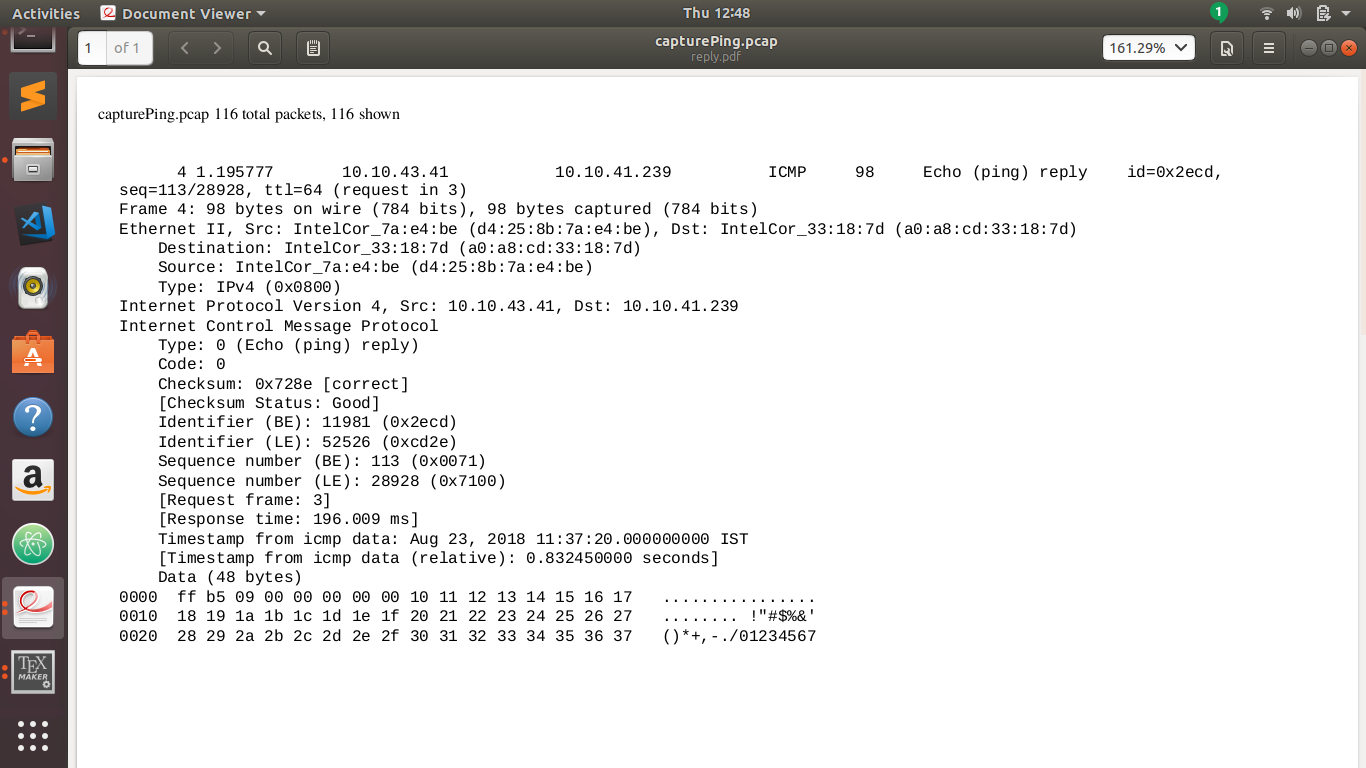
\includegraphics[width=0.7\textwidth]{../Q4/reply.png}
 \caption{\label{fig:REPLY}Ping reply}
 \end{figure}

 
\section{Q5: tcpdump −enx −w exe5.out}
We will not be able to see anything on the terminal screen as all the output of tcpdump command is being written on exe5.out file

\section{Q6: tcpdump −enx −w exe5.out}

\begin{figure}[H]
 \centering
 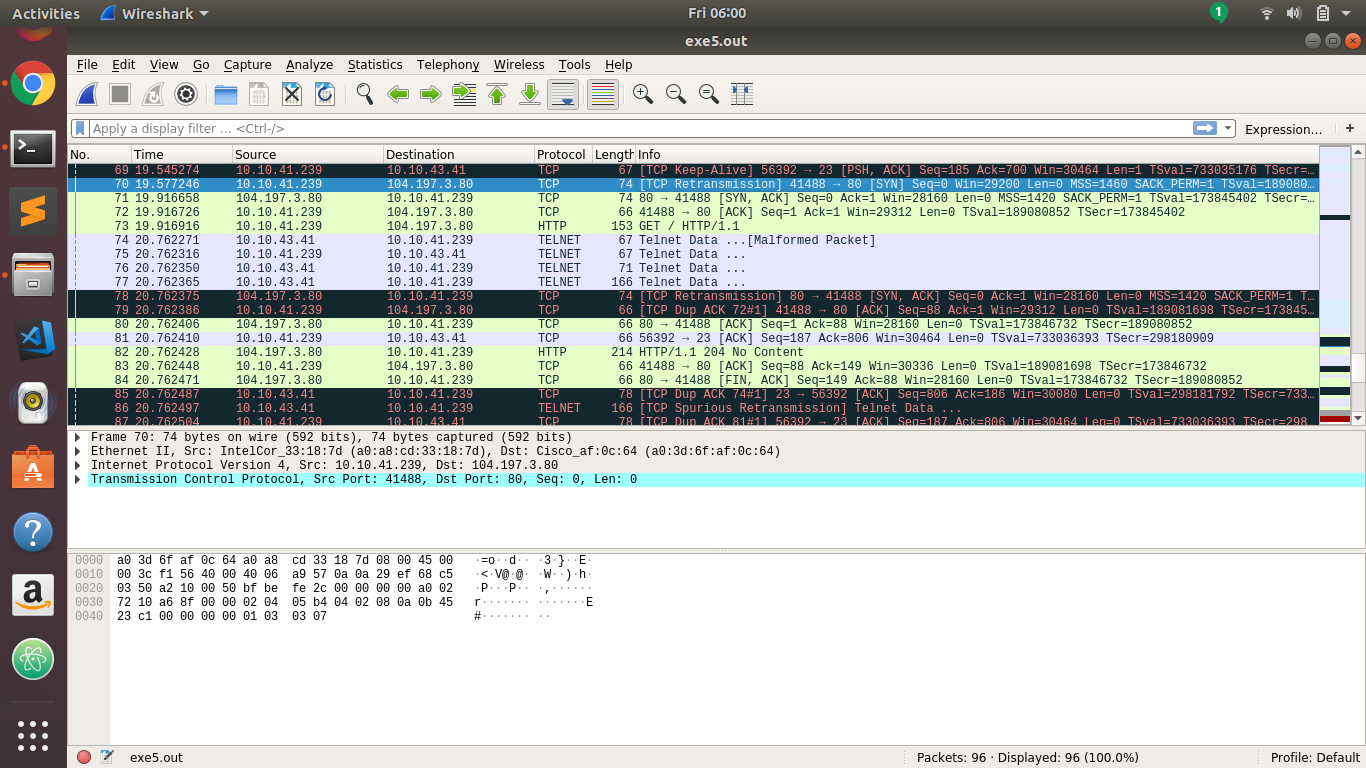
\includegraphics[width=1.0\textwidth]{../Q6/exe5.png}
 \caption{\label{fig:EXE5.OUT}Screnshot of Tcpdump file.}
 \end{figure}
 \begin{figure}[H]
 \centering
 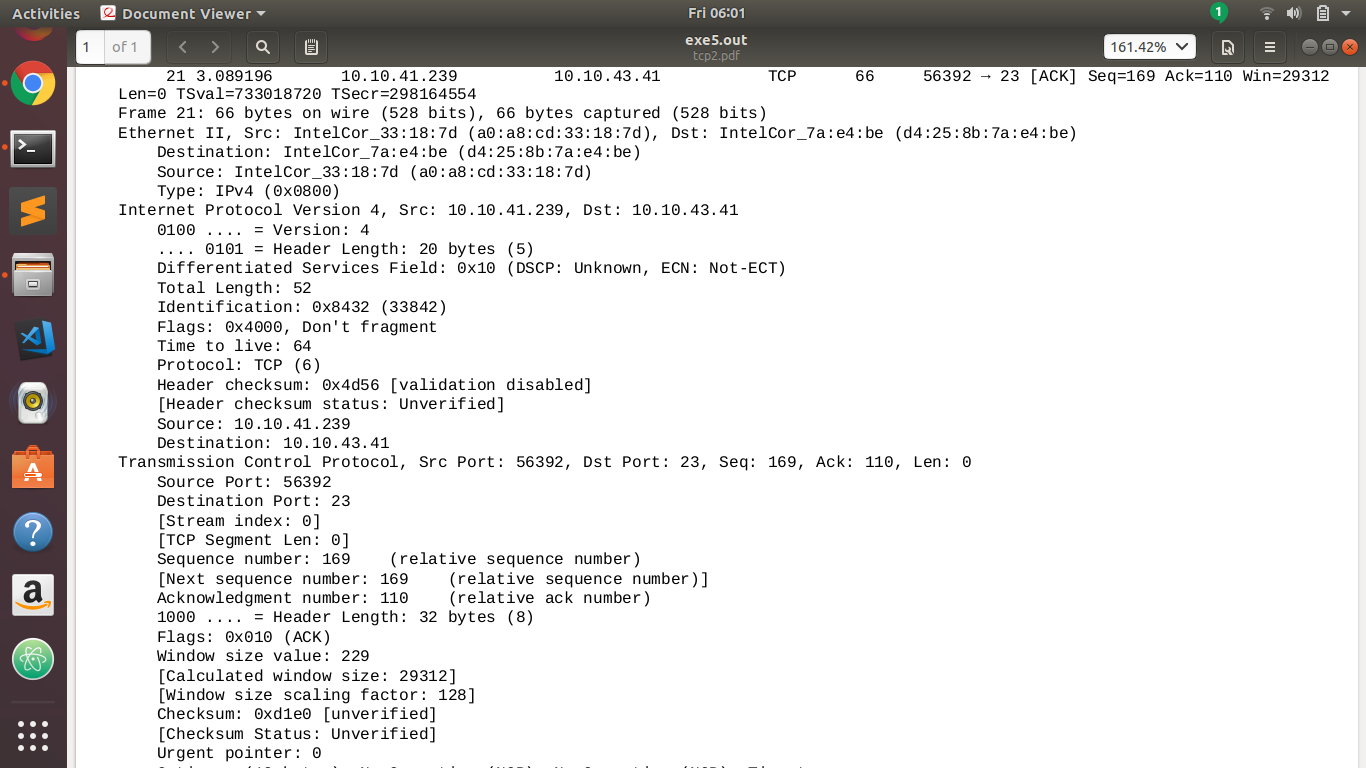
\includegraphics[width=1.0\textwidth]{../Q6/tcp2.png}
 \caption{\label{fig:Tcp Packet}Screenshot of a tcp packet.}
 \end{figure}
\subsection{A}
\begin{table}[H]
\begin{center}
\caption{IP header format}
\label{tab:table1}
\scalebox{0.9}{
\begin{tabular}{ | c | c | c | c | c | c | }
\hline
Version:0100....&Hdrlen 20bytes&DifrentiatedServices:0x10(16)&\multicolumn{3}{c|}{TotalLength:53}\\
\hline
\multicolumn{3}{|c|}{Identification:0x8432(33842)}&Flag:0x4000(16384)&\multicolumn{2}{c|}{FragementOffset:0}\\
\hline
\multicolumn{2}{|c|}{TimeToLive:64}&Protocols:TCP&\multicolumn{3}{c|}{HeaderCheckSum:0x3fed}\\
\hline
\multicolumn{6}{|c|}{Source IP Address:10.10.41.239}\\
\hline
\multicolumn{6}{|c|}{Destination IP Address:10.10.43.41}\\
\hline
\multicolumn{6}{|c|}{Options:}\\
\hline
\multicolumn{6}{|c|}{Data}\\
\cline{1-6}
\end{tabular}
}
\end{center}
\end{table}

\begin{table}[H]
\begin{center}
\caption{TCP header format}
\label{tab:table2}
\scalebox{1.0}{
\begin{tabular}{ | c | c | c | c | c | c | }
\hline
\multicolumn{3}{|c|}{Source Port Number:56392}&\multicolumn{3}{c|}{Destination Port Number:23}\\
\hline
\multicolumn{6}{|c|}{Sequence Number:169}\\
\hline
\multicolumn{6}{|c|}{Acknowledgement Number:110}\\
\hline
Hdr Len:32 bytes&Reserved:Not Set&Flags:0x010(16)(ACK)&\multicolumn{3}{|c|}{Window Size:229}\\
\hline
\multicolumn{3}{|c|}{Tcp CheckSum:0xd1e0(53728)}&\multicolumn{3}{|c|}{Urgent Pointer:0}\\
\hline
\multicolumn{6}{|c|}{Options:}\\
\hline
\multicolumn{6}{|c|}{Data:}\\
\cline{1-6}
\end{tabular}}
\end{center}
\end{table}

\begin{table}[H]
\begin{center}
\caption{Link header format}
\label{tab:table3}
\scalebox{0.9}{
\begin{tabular}{ | c | c | c | c | c | c | }
\hline
$IntelCor_33:18:7d$ (a0:a8:cd:33:18:7d)&$IntelCor_7a:e4:be$ (d4:25:8b:7a:e4:be)&FT:IPv4&\multicolumn{2}{c|}{Data}&CRC\\
\cline{1-6}
\end{tabular}}
\end{center}
\end{table}

\subsection{B}
TCP 6 .The Protocol field in the IPv4 header contains a number indicating the type of data found in the payload portion of the datagram. The most common values are 17 (for UDP) and 6 (for TCP). This field provides a demultiplexing feature so that the IP protocol can be used to carry payloads of more than one protocol type.

\section{Q7: ARP}
 \begin{figure}[H]
 \centering
 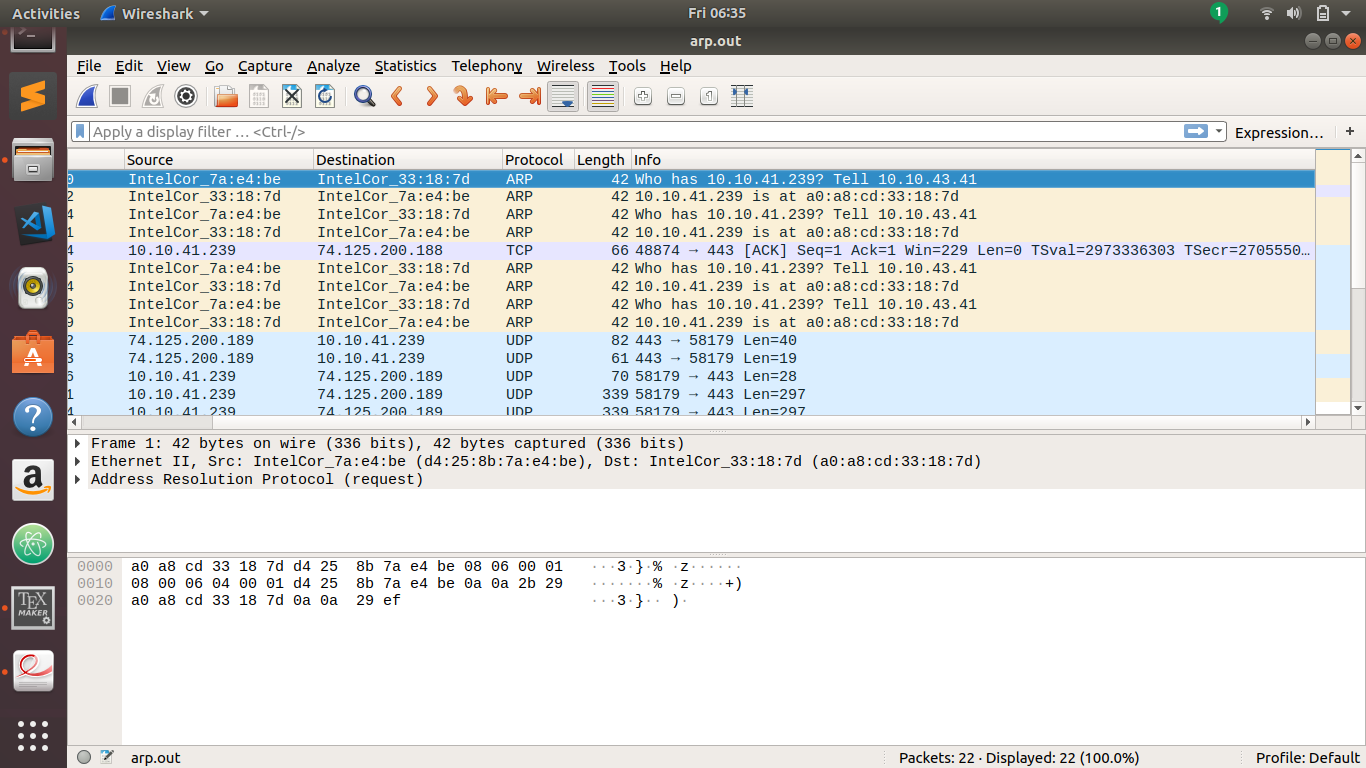
\includegraphics[width=1.0\textwidth]{../Q7/arp.png}
 \caption{\label{fig:ARP}Screenshot of tcpdump file.}
 \end{figure}
\subsection{Request}
\begin{figure}[H]
 \centering
 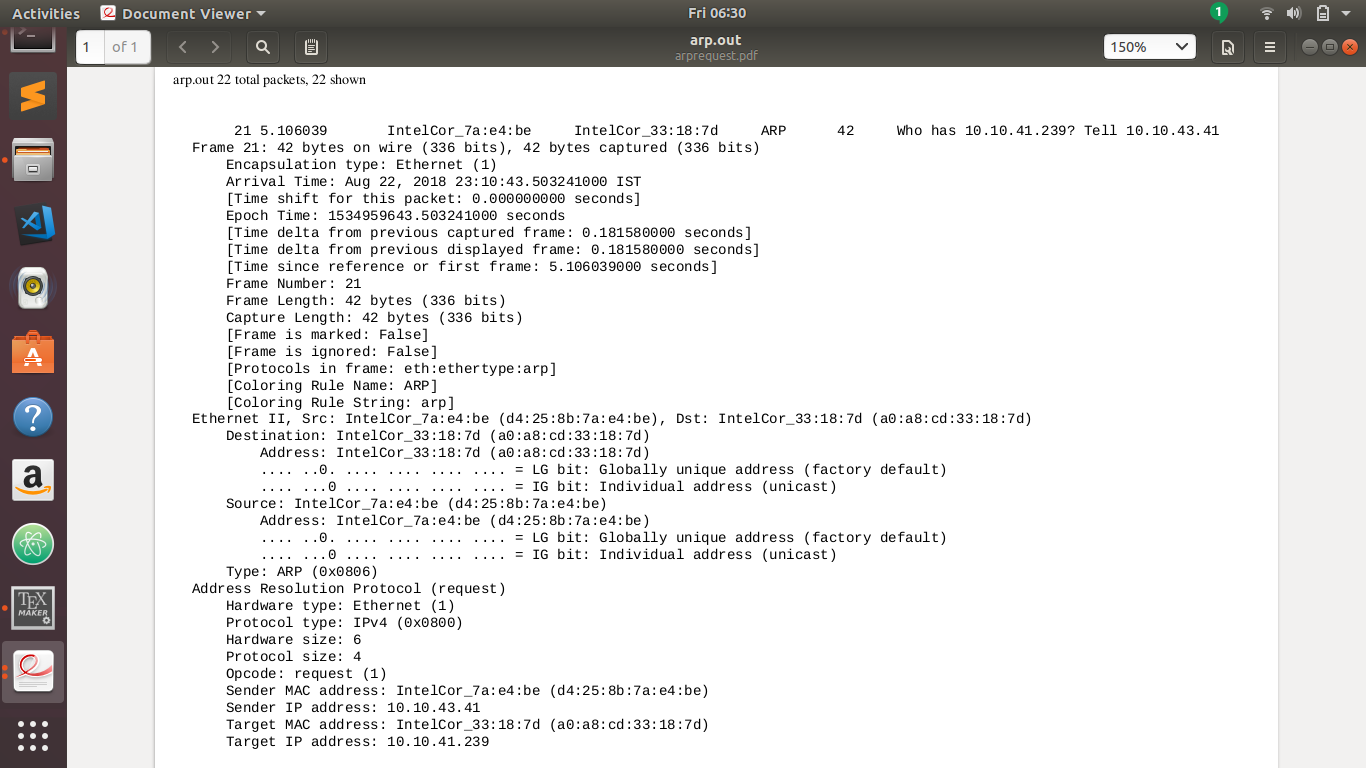
\includegraphics[width=1.0\textwidth]{../Q7/request.png}
 \caption{\label{fig:REQUEST}Arping request}
 \end{figure}
\subsection{Reply}
 \begin{figure}[H]
 \centering
 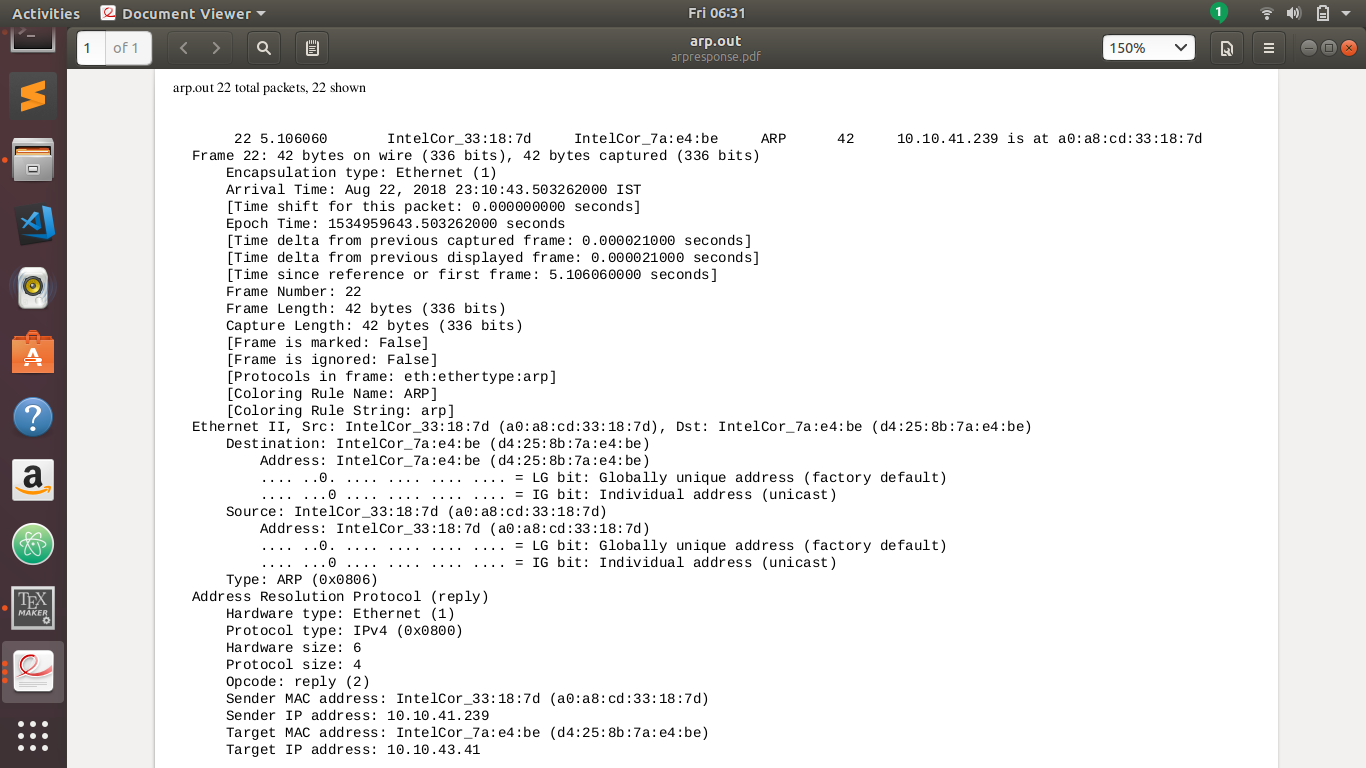
\includegraphics[width=1.0\textwidth]{../Q7/response.png}
 \caption{\label{fig:REPLY}Arping reply.}
 \end{figure}
\subsection{A}
REQUEST Type: ARP 0x0806(2054) \\
REPLY Type:  ARP 0x0806(2054)
\subsection{B}
Type: IPv4 0x0800 (2048)
\subsection{C}
It is used to indicate which protocol is encapsulated in the payload of the frame. The same field is also used to indicate the size of some Ethernet frames

\section{Q8: TCPDUMP Expressions}
\subsection{tcpdump udp port 520}
UDP Port 520 may use a defined protocol to communicate depending on the application. UDP port 520 uses the Datagram Protocol, a communications protocol for the Internet network layer, transport layer, and session layer. This protocol when used over PORT 520 makes possible the transmission of a datagram message from one computer to an application running in another computer.
\subsection{tcpdump -x -s 120 ip proto 89}
To capture OCPF Packets with size 120 bits.Open Shortest Path First (OSPF) is a routing protocol for Internet Protocol networks. It uses a link state routing algorithm and falls into the group of interior gateway protocols, operating within a single autonomous system.
\subsection{tcpdump -x -s 70 host ip addr1 and (ip addr2 or ip addr3)}
To capture packets and trim down to size 70 bits either to and fro from IP1 or IP2.
\subsection{tcpdump -x -s 70 host ip addr1 and not ip addr2}
To capture packets where IP addr1 is either src or dst and IP addr2 is neither of src and dest . Also to trim packets to 70 bits.
\section{Q9: tcpdump -n -nn host your host and remote host}
\begin{figure}[H]
 \centering
 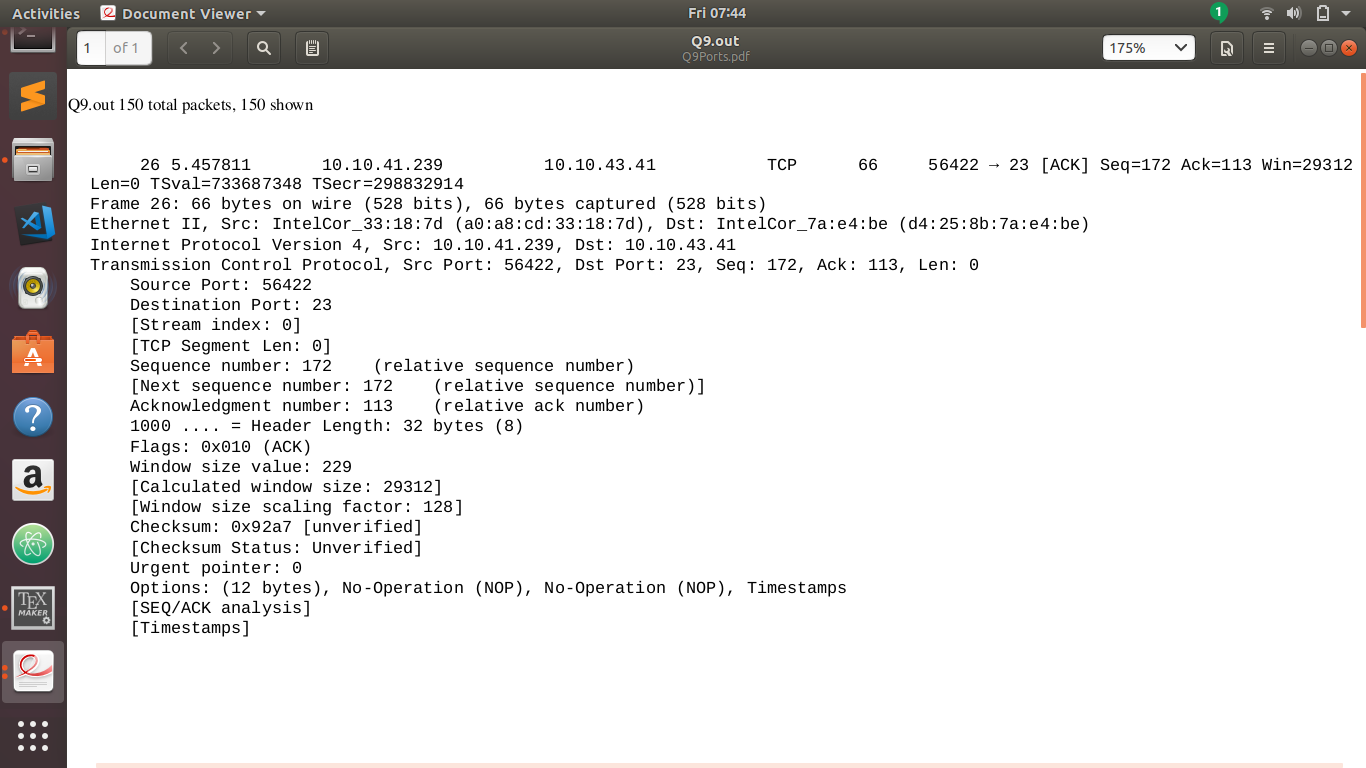
\includegraphics[width=1.0\textwidth]{../Q9/ports.png}
 \caption{\label{fig:PORTS}Screenshot of tcpdump packet}
 \end{figure}
\subsection{port numbers used by the remote and the local computer}
Remote Port No : 23 \\
Local Port No : 56422
\subsection{Which machine  port number matches the port number listed for telnet in the /etc/services file}
Remote machine port no matches with the port number listed for telnet (23) in etc/services file

\section{Q10: tcpdump -n -nn host your host and remote host}
\begin{figure}[H]
 \centering
 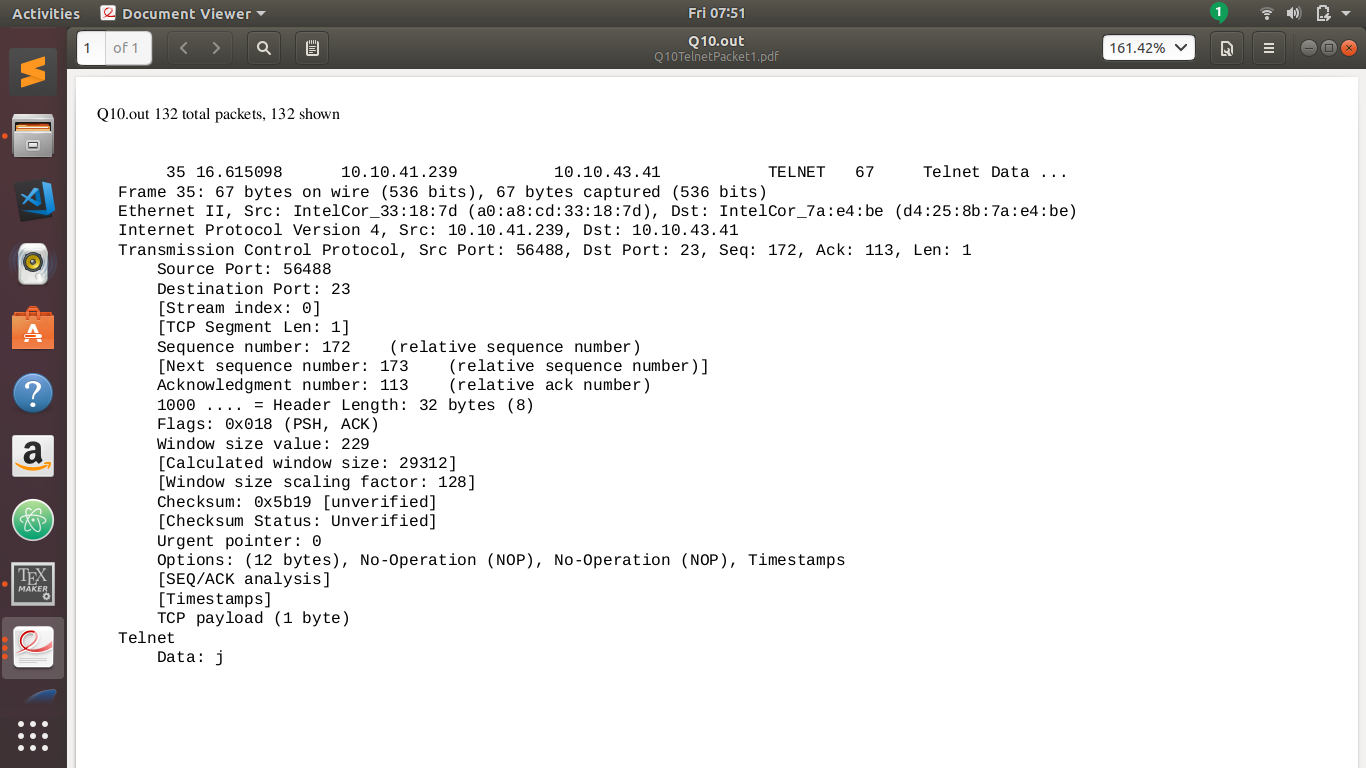
\includegraphics[width=1.0\textwidth]{../Q10/packet1.png}
 \caption{\label{fig:PACKET1}Screenshot of packet1.}
 \end{figure}
 \begin{figure}[H]
 \centering
 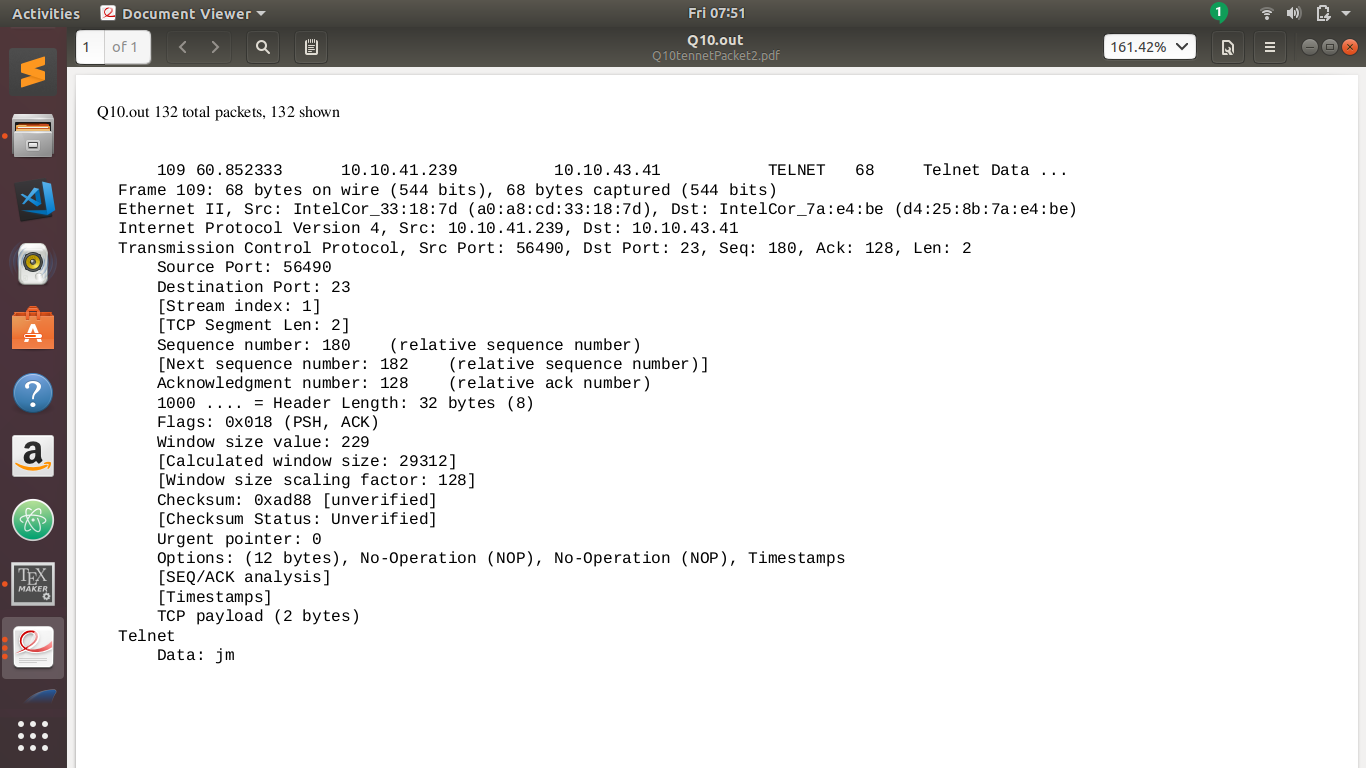
\includegraphics[width=1.0\textwidth]{../Q10/packet2.png}
 \caption{\label{fig:PACKET2}Screenshot of packet2.}
 \end{figure}
\subsection{A}
Remote Machine Port No : 23 \\
Yes both sessions are connected to the same port number on the remote machine.
\subsection{B}
1st Telnet session Local Machine Port No : 56488 \\ 
2nd Telnet session Local Machine Port No : 56490
\subsection{C}
Internet-wide port number : 0 - 1023 \\
For linux systems         :  1 - 60179 \\
client port numbers       : 1024 - 65535 \\
The ports in etc/services differ from 1 - 60000 range. Hence the client port number are not consistent.



\end{document}